\section{Simulación en Cadenas de Espines}

En esta sección exploramos una conexión entre el tratamiento de campo medio de pares investigado en primer lugar (capítulos \ref{ch:cm}, \ref{ch:dim1} y \ref{ch:dim2}) con el formalismo de tiempo desarrollado en los capítulos \ref{ch:st} y \ref{ch:his}. Mostraremos que eligiendo una partición adecuada de la cadena de espines dimerizada, es posible simular estados historia de manera eficiente.

\begin{figure}[htp]
\centering
\includegraphics[width=0.6\textwidth]{%Figures/
dimclock.pdf}
\caption{Esquema que representa la simulación de un estado historia en una cadena de espines dimerizados.} 
\label{fig:dimerclock}
\end{figure}

Consideremos una cadena cíclica de 2n espines $s$ y una partición de la misma compuesta por los n espines ``externos'' y los n espines ``internos (es decir, los n izquierdos y los n derechos de cada dímero), como se aprecia en la figura \ref{fig:dimerclock}. El estado fundamental puede siempre escribirse 
como 
\begin{equation}
    |\Psi\rangle=\sum_{J,L}C_{JL}|J\rangle|L\rangle
\end{equation}
donde $|J\rangle$ y $|L\rangle$ denotan estados de una base ortonormal arbitraria para el sistema de $n$ espines internos y externos respectivamente. Mediante la correspondiente descomposición de Schmidt, este estado puede reescribirse  como (ver (\ref{Scm})) 
\begin{equation}|\Psi\rangle=\sum_K  \sqrt{P_K}|K_I\rangle|-K_E\rangle\label{SK}\end{equation}
donde $P_K$ y los estados ortogonales  $|K_{I(E)}\rangle$ se obtienen a partir de la descomposición en valores singulares de  la matriz $C_{JL}$. Estos valores $P_K$ coinciden por su puesto con los autovalores de la matrices densidad reducidas $\rho_{I(E)}={\rm Tr}_{E(I)}\,|\Psi\rangle\langle\Psi|$. 

A partir de (\ref{SK}) y la {\it DFT} de los estados de Schmidt, puede obtenerse,  como se discutió previamente (ver (\ref{St2})),  un estado de historia ``externo-interno'', donde uno de ellos puede interpretarse como reloj:
\begin{equation}
    |\Psi\rangle=\sum_{\tau}\frac{1}{d^{n/2}}\exp[-iH_I\tau]|I_0\rangle
    |\tau\rangle
\end{equation}
donde $|\tau\rangle\equiv\frac{1}{\sqrt{d^n}}\sum_K e^{-i2\pi K\tau/d^n}|K_E\rangle$   son estados ortonormales del ``reloj'' E, con $d=2s+1$,  $\tau=0,\ldots,d^n-1$,  $H_I|K_I\rangle=(2\pi K/d^n)|K_I\rangle$ y 
$|I_0\rangle=\sum_K\sqrt{P_K}|K_I\rangle$ es el estado inicial efectivo del sistema $I$.  

En el caso general, los estados locales de la base de Schmidt $|K_{E}\rangle$ y $|K_I\rangle$ son estados complejos entrelazados de $n$ espines. 
Notablemente, en el caso de una cadena dimerizada en una fase dimerizada, que, como vimos, puede ser descripta muy satisfactoriamente por medio de la aproximación de campo medio de pares, 
tal estado se simplifica considerablemente: 
El estado global de la cadena tiene la forma de un producto de estados de pares, 
\begin{equation}
|\Psi\rangle=\otimes_{i=1}^n|\psi_i\rangle\,
\end{equation}
con $|\psi_i\rangle$ el estado del par $i$ (que por simplicidad de notación consideraremos independiente de $i$, como en el caso de una cadena dimerizada uniforme):
\begin{equation}|\psi_i\rangle=\sum_{k}\sqrt{p_k}|k_I\rangle|-k_E\rangle\,.\end{equation}
Aquí hemos utilizado la descomposición de Schmidt del estado del par, con $k=1,\ldots,d$ y $d=2s+1$ para el caso de un par de espines $s$. 

As\'{\i}, la descomposición de Schmidt (\ref{SK}) toma la forma 

\begin{equation}
    |\Psi\rangle=\sum_{k_1\ldots,k_n}
    \sqrt{p}_{k_1}\ldots\sqrt{p}_{k_n}|k_{1I}\ldots k_{nI}\rangle|-k_{1E}\ldots -k_{nE}\rangle\,.
\end{equation}
Esto es, los estados de Schmidt locales son precisamente estados producto de los $n$ espines $I$ o $E$. En otras palabras, los estados $|K_E\rangle=|k_{1E}\ldots k_{nE}\rangle$, 
con $k_i=1,\ldots, 2s+1$,  $K=1,\ldots d^n$, 
forman una base producto, con $K$ expresado en notación de base $d=2s+1$ (binaria si $s=1/2$, ``ternaria'' si $s=1$, etc.). A partir de esta expresión, los estados locales de tiempo son la {\it DFT} de estos estados locales $|K_E\rangle$. El entrelazamiento ``sistema-tiempo'' toma la forma 
$E(S,T)=n S(|\psi_i\rangle)$, con $S(|\psi_i\rangle)=-\sum_k p_k \log_2 p_k$ 
el entrelazamiento de un par. 

En particular, si el estado del par es máximamente entrelazado, $p_k=1/\sqrt{2s+1}$ 
$\forall$ $k$, entonces $|\Psi\rangle$ es m\'aximamente entrelazado en esta partición, y por ende cualquier base %producto 
local $|K_E\rangle$ resulta en este caso equivalente. 

Esto muestra que una cadena de espines puede ser utilizada para simulación de estados historia, con una dimensión que crece exponencialmente con el número $n$ de pares. 


\section{Simulación de Estados Historia por Medios Ópticos\label{sec:impl}}

En esta sección se discute una simulación
la simulación de estados historia discretos
utilizando una arquitectura completamente óptica.
Esta investigación se realizó
en colaboración con el laboratorio
de Procesado de Imágenes del Departamento de Física de la Facultad de Ciencias Exactas
de la Universidad de Buenos Aires \cite{OP}. 

Con este fin, se utilizó el momento transverso lineal 
de fotones individuales para representar al tiempo $|t\rangle$ del sistema cuántico reloj $T$, 
y su polarización lineal para codificar al estado $|S_t\rangle$ del sistema cuántico $S$.


\begin{figure}[htp]
\centering
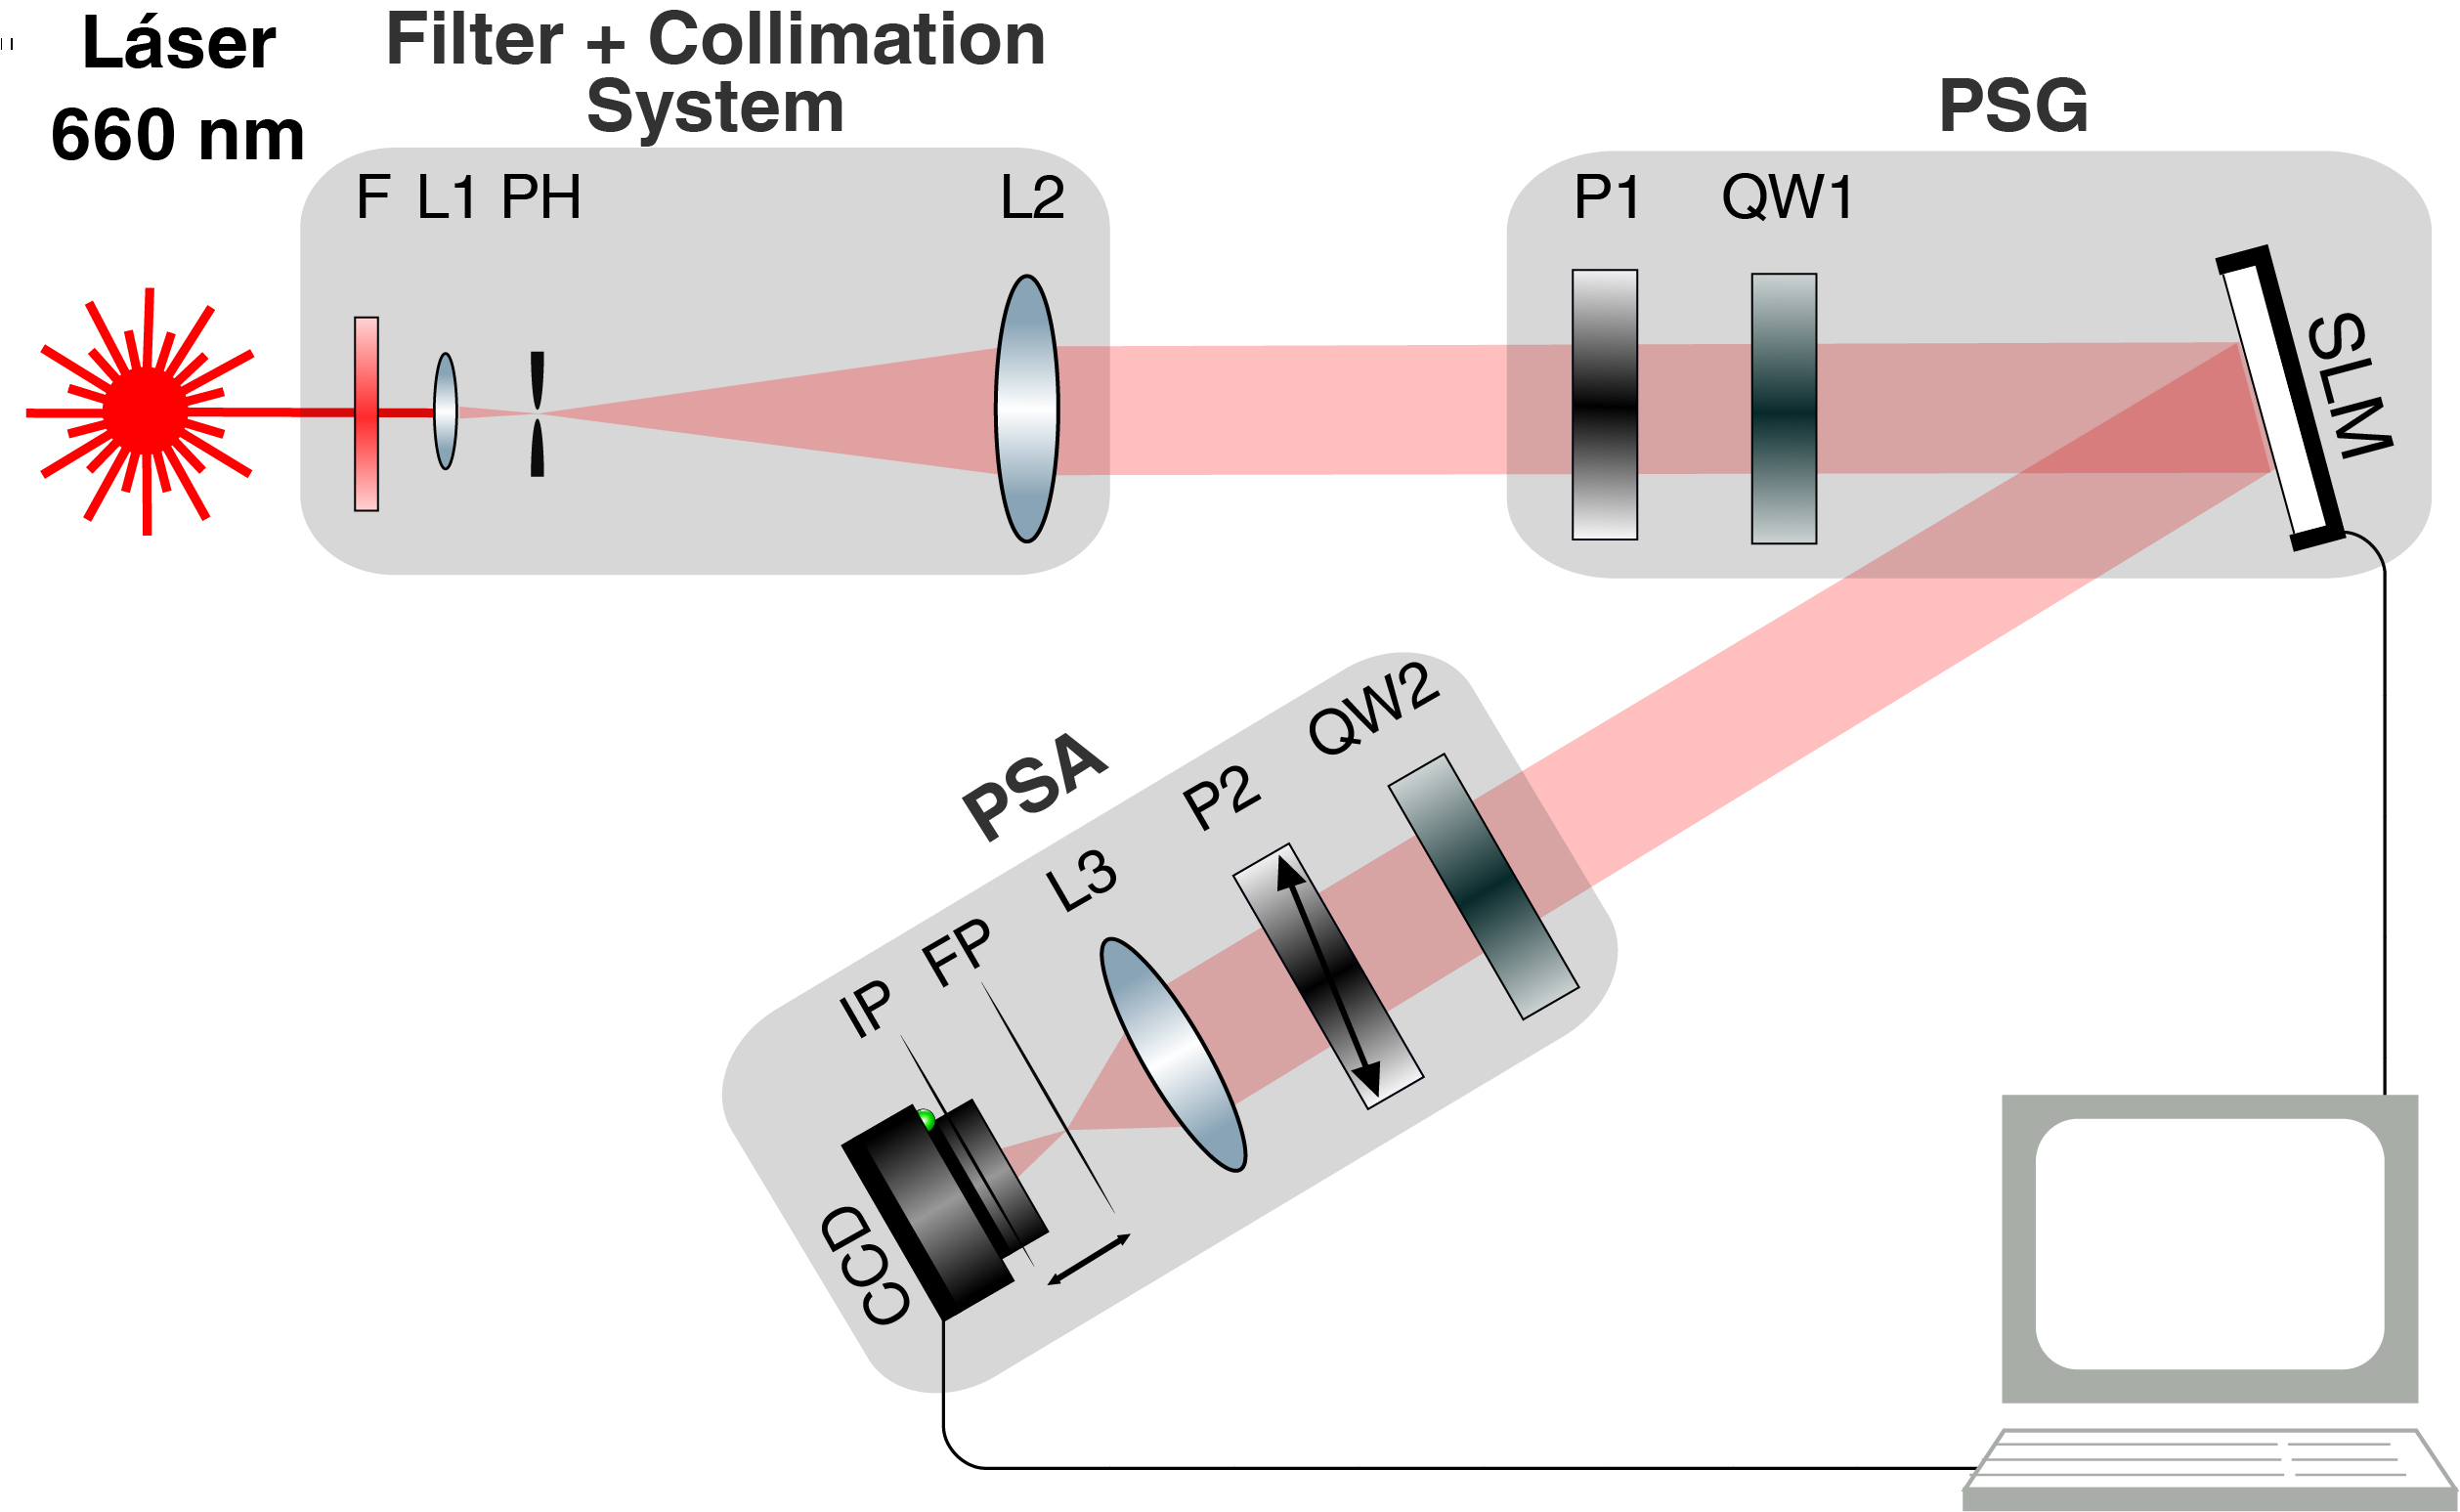
\includegraphics[width=0.8\textwidth]{SETUP.jpg}
\caption{Generación y caracterización de estados historia.} 
\label{fig:setup}
\end{figure}

El arreglo experimentar para simular evolución
cuántica paralela en el tiempo se presenta en la  Fig.~\ref{fig:setup}. En la primera parte, 
se ilumina con un láser de estado sólido de $660\text{nm}$,
el cual es filtrado y colimado de forma tal que incida en un 
modulador espacial de luz programable ({\it Spatial Light Modulator:} $\text{SLM}$) con una onda plana de fase aproximadamente constante y amplitud distribuida sobre la región de interés ({\it Region Of Interest: ROI}). 
Este SLM, basado en un micro-display de {\it Liquid Crystal-on-Silicon: (LCoS)} reflectivo, con una resolución 
espacial de 1024x768 píxeles, se emplea para representar al estado historia $|\Psi\rangle$, dando la posibilidad de modificar dinámicamente la función óptica en la pantalla, píxel a píxel.
En particular, el SLM utilizado en nuestro experimento,
está formado por un {\it HoloEye Lc-R 2500} 
en combinación con un polarizador (P1) 
y una placa de cuarto de onda (QW1) 
que provee el estado de luz
polarizada incidente adecuado 
para alcanzar la amplitud máxima
y modulación de fase entre dos polarizaciones ortogonales~\cite{marquez2001,marquez2008}.  %{\color{red} (ver si van estas Refs.)}. 
Esto nos permite tener un amplio rango de modulación de polarización para la cual la amplitud del campo electromagnético se mantiene constante,
independientemente del nivel de gris para el cual se configuran los píxeles del {\it LCoS}. A su vez, para este estado inicial,
no hay fase inicial adicional en el estado de salida debida al 
camino óptico. %In Fig.~\ref{fig:sphere} we see the output polarization states accessible trough the SLM when the input beam is prepared in a particular state elliptically polarized. Each point on the Bloch sphere corresponds to the particular grey level, between 0 and 255, addressed on the SLM.

%\begin{figure}[htp]
%\centering
%\includegraphics[width=0.30\textwidth]{Figures/Sphere1.pdf}
%\caption{Accessible polarization states }
%\label{fig:sphere}
%\end{figure}


Finalmente, dado que cada píxel se puede controlar de forma individual, se puede programar una función particular $f(\mathbf{x})$ 
que caracteriza la distribución de modulación. Luego, 
el frente de onda del campo adquiere una polarización específica condicionada por la posición transversal al plano del {\it SLM}. En la  Fig.~\ref{fig:schematic-codification} 
se muestra, esquemáticamente, un ejemplo de esto cuando se configuran ocho regiones rectangulares independientes en la pantalla del {\it  SLM}, cada una con un nivel de gris constante particular. 


\begin{figure}[htp]
\centering
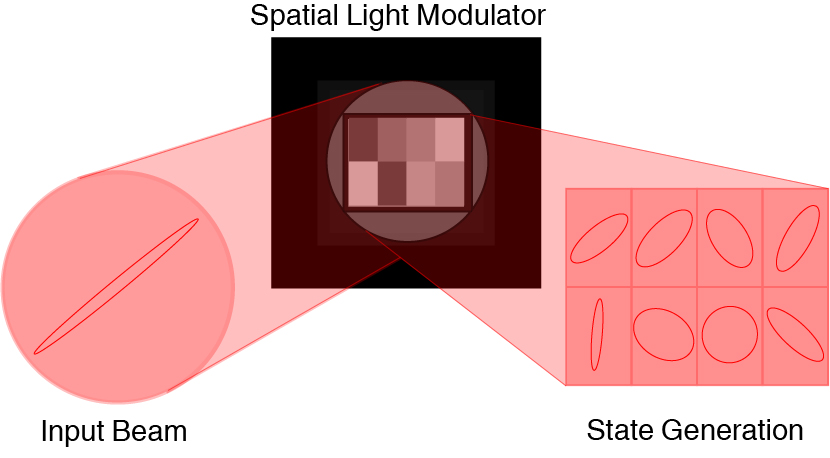
\includegraphics[width=0.8\textwidth]{SLM.jpg}
\caption{{\color{red} }} 
\label{fig:schematic-codification}
\end{figure}



En la segunda parte del arreglo experimental, se utiliza un analizador de polarización del estado ({\it Polarization State Analyzer: PSA})
para la caracterización del {\it SLM}
como un generador de estados en polarización ({\it Polarization State Generator: PSG}). 
Con este fin, se dispuso un nivel de gris constante en toda la pantalla. Luego de reflejar en el {\it SLM}, el haz saliente se enfocó por medio de la lente {\it L3} 
en el plano de detección del fotodiodo,
que no se muestra aquí. %high sensitive camera based on CMOS
%technology {\color{red}(ver)}. %The camera used is an Andor
%Zyla 4.2 sCMOS.
La placa de cuarto de onda (QW2) 
y el polarizador lineal (P2) 
proyectan al estado inicial del fotón 
en distintas bases, mientras que medidas de intensidad se registran en el plano imagen (IP). Esto permite la completa reconstrucción de las matrices de Mueller 
del {\it SLM} a partir de las cuales se puede obtener la intensidad de modulación para cada nivel de gris.
En la Fig.~\ref{fig:sphere} 
se presenta los estados de salida de polarización
accesibles a través del {\it SLM}
cuando el haz incidente es preparado en un estado particular con polarización elíptica.
Cada punto en la esfera de
Bloch corresponde a un único nivel de gris, entre 0 y 255, configurado en el {\it SLM}.
Asimismo, se realizaron medidas de interferencia en el plano de Fourier (FP), 
entre los haces provenientes de dos regiones del {\it SLM}
configuradas con diferentes niveles de gris. %Con esta información adicional se

%With this additional information we obtained the phase modulation introduced by the SLM by means of the Jones calculus {\color{red} (Ref.)}.
\begin{figure}[htp]
\centering
\includegraphics[width=0.6\textwidth]{Sphere1.pdf}
\caption{Estados de polarización accesibles.}
\label{fig:sphere}
\end{figure}

%%%%%%%%%%%%%%%%%%%%%%%%%%%%%%%%%%%%%%%%%%
Una vez que hemos caracterizado completamente al {\it SLM},
el mismo sistema {\it PSG-PSA} se empleó para simular experimentalmente distintos estados
historia sistema-tiempo discretos 
$|\Psi\rangle$, 
y la subsecuente  evolución unitaria del estado del sistema $|S_t\rangle=U_{t}|S_0\rangle$ 
($t=0,...,N-1$). 


\subsection{\label{sec:state_generation} Generación de Estados Historia Discretos}

Como hemos visto en el capítulo \ref{ch:st}, el estado historia 
$|\Psi\rangle$ se puede generar a partir de un estado inicial producto $|S_0\rangle|0\rangle$ 
como
\begin{equation}\label{Eq:histGen}
    |\Psi\rangle=\mathcal{W}(\mathbbm{1}\otimes H)|S_0\rangle|0\rangle \,.
\end{equation}

% donde $H$  es una compuerta Hadamard
% que actúa en el sistema reloj $\big(H|0\rangle= \frac{1}{\sqrt{N}} \sum_{t=0}^{N-1}|t\rangle \big)$ and 
% $\mathcal{W}=\sum_{t=0}^{N-1} U_t{\otimes }|t\rangle\langle t|$
% is the control-$U_t$ gate. For $t=0,1,...,N-1$, the $U_t~'s$ are unitary operators on the system $S$, so that
% $|S_t\rangle=U_t|S_0\rangle$. 

En la implementación experimental, 
el estado inicial total es un estado fotónico definido por 
el producto entre su estado de polarización ($|S_0\rangle$)
y su estado espacial $(|0\rangle)$ 
descripto por el perfil transversal del frente de onda .
El tratamiento, tanto de la polarización como del grado de libertad espacial de los fotones en la utilización del {\it SLM}, se enmarcó dentro de un formalismo similar al empleado en \cite{solis2013,lemos2014}. 

% to manipulate the polarization or the transverse spatial DOF of photons trough the use of SLMs, the generation of history states can be explained as follows:
% La generación de estados historia se puede e

Con el fin de simular la generación de estados historia asumimos que el campo del fotón individual es paraxial y monocromático, considerándolo descripto por un estado puro
\begin{equation}
|S_0\rangle|0\rangle=\sum_{\mu}\int\!d\mathbf{x}\,\alpha_\mu\psi(\mathbf{x})|\mu\rangle|1\mathbf{x}\rangle,
\end{equation}
donde $\mu$
barre dos polarizaciones ortogonales, $\mathbf{x}=(x,y)$ 
es la coordenada de la posición transversal, y $\psi(\mathbf{x})$ 
es la amplitud de probabilidad transversal normalizada 
para este estado:  $\int\!d\mathbf{x}\,|\psi(\mathbf{x})|^2=1$. 
El {\it SLM} introduce
una modulación dependiente de la polarización que 
puede ser idealmente interpretado como la acción del operador
%After impinging the SLM, programmed with a polarization dependent modulation distribution $f_{\mu\nu}(\mathbf{x})$, where $\mu, \nu$ are polarization indices,
\begin{equation}
    \hat{f}=\sum_{\alpha, \beta}\int d\mathbf{x}f_{\alpha \beta}(\mathbf{x})|\alpha,1 \mathbf{x}\rangle\langle\beta, 1\mathbf{x}|,
\end{equation}
tal que, luego de atravesar el {\it SLM},
el estado del fotón es
\begin{equation}
|\Psi\rangle\propto\sum_{\mu,\nu}\label{Eq:transf} \int\!d\mathbf{x}\,\alpha_\nu\psi(\mathbf{x})f_{\mu\nu}(\mathbf{x})|\mu\rangle|1\mathbf{x}\rangle.
\end{equation}

Consideremos una distribución de modulación $f_{\mu\nu}(\mathbf{x})$,
la cual define una matriz de $N$ regiones espaciales adyacentes de ancho $2a$, 
y largo $2b$. En cada una de estas regiones se tiene una modulación compleja constante, $C_{\mu\nu}^{(t)}$. Luego,
\begin{equation} \label{eq:fNregions}
\begin{split}    
f_{\mu\nu}(\mathbf{x})&= \sum_{t=0}^{N-1}C_{\mu\nu}^{(t)}~{\rm
rect}\!\left(\frac{x-x_t}{2a}\right){\rm
rect}\!\left(\frac{y-y_t}{2b}\right)\\
&C_{\mu\nu}^{(t)}=c_{\mu\nu}^{(t)}{\rm e}^{i\phi^{(t)}_{\mu\nu}},~~c_{\mu\nu}^{(t)}\geq0
\end{split}
\end{equation}
donde ${\rm
rect}\!\left(u\right)=1$ si $|u| < \frac{1}{2}$, 0 en caso contrario, y 
los centros de estas regiones están en $\{(x_t,y_t)\}_{t=0}^{N-1}$, con $x_t=a, 3a,5a,...,$ y $y_t=b, 3b, 5b,...$ 

Sin pérdida de generalidad y en acuerdo con las condiciones del experimento, podemos
asumir que  $\psi(\mathbf{x})$ es constante 
a lo largo de la región de interés ({\it ROI}). Por lo que podemos reescribir al estado (\ref{Eq:transf}) como

% \begin{equation}
% \begin{split}
% \frac{1}{\sqrt{A_{ROI}}}&\sum_{t=0}^{N-1}\mathop{\int}_{ROI}d\mathbf{x}\,{\rm
% rect}\!\left(\frac{x-x_t}{2a}\right){\rm
% rect}\!\left(\frac{y-y_t}{2b}\right)|1\mathbf{x} \rangle\\
% &=\frac{1}{\sqrt{N}}\sum_{t=0}^{N-1}|t\rangle,
% \end{split}
% \end{equation}
% con
% $|t\rangle=\frac{1}{\sqrt{A_t}}\int d\mathbf{x}\,{\rm
% rect}\!\left(\frac{x-x_t}{2a}\right){\rm
% rect}\!\left(\frac{y-y_t}{2b}\right)|1\mathbf{x}\rangle$.   
% Como las regiones espaciales definidas en el {\it SLM} tienen {\it overlap} despreciable, 
% estos $N$ estados $\left\lbrace |t\rangle\right\rbrace_{t=0}^{N-1}$, forman una base 
% ortonormal del espacio de Hilbert para la coordenada de la posición transversal
% del fotón individual. De esta forma, podemos simular la acción de la compuerta Hadamard $H$, 
% sobre el estado inicial del sistema reloj. Finalmente, combinando este resultado con la Ec.~(\ref{eq:fNregions}), el estado transformado en la Ec.~(\ref{Eq:transf}) se puede
% escribir como  

\begin{equation}
|\Psi\rangle\propto\sum_{t=0}^{N-1}\sum_{\mu,\nu}\alpha_\nu C_{\mu\nu}^{(t)}|\mu\rangle|t\rangle,\label{Psi_mod} 
\end{equation}
donde $|t\rangle=\frac{1}{\sqrt{A_t}}\int d\mathbf{x}\,{\rm rect}\!\left(\frac{x-x_t}{2a}\right){\rm rect}\!\left(\frac{y-y_t}{2b}\right)|1\mathbf{x}\rangle$. 

En la implementación experimental, la modulación introducida por el {\it SLM}
implica solamente una transformación en el grado de libertad de polarización. Esto significa que $\sum_{\mu,\nu}\alpha_\nu C_{\mu\nu}^{(t)}|\mu\rangle|t\rangle= (U_t\otimes\mathbbm{1})|S_0\rangle|t\rangle\equiv |S_t\rangle|t\rangle$, con $U_t$ 
una matriz unitaria tal que  $|S_t\rangle=U_t|S_0\rangle=\sum_{\mu,\nu}\alpha_\nu C_{\mu\nu}^{(t)}|\mu\rangle$ es el estado de polarización asociado a la región  $t$. Luego, el {\it SLM} transforma al estado inicial del fotón 
de la siguiente forma: 
\begin{equation}
\begin{split}
|S_0\rangle|0\rangle\stackrel{\rm{SLM}}{\Longrightarrow}~& \frac{1}{\sqrt{N}}\sum_{t=0}^{N-1}U_t|S_0\rangle|t\rangle={\cal W}\left(|S_0\rangle\sum_{t=0}^{N-1}\frac{1}{\sqrt{N}}|t\rangle\right)\\
&={\cal W}\left(\mathbbm{1}\otimes H\right)|S_0\rangle|0\rangle\,,
\end{split}
\end{equation}
generando por lo tanto  al estado historia (\ref{Eq:histGen}), donde el sistema $S$ 
y el sistema reloj $T$ son emulados a través de la polarización y el grado de libertad espacial, respectivamente.

%In terms of quantum evolution, each modulation distribution, $f(\mathbf{x})$, as given in Eq.~\ref{eq:fNregions}, defines an unitary operator on the transverse spatial degree of freedom (DOF): $\Lambda_f\equiv\sum_{t=0}^{N-1}\tilde{f}_t|t\rangle\langle t|$, with $\tilde{f}_t=f_t/\sqrt{\sum_{t=0}^{N-1}|f_t|^2}$. In the space defined by polarization and transverse spatial DOFs, the action of the SLM can be described, ideally, as \begin{eqnarray}
%|p_+\rangle\langle p_+|\otimes\Lambda_{f^+}+|p_-\rangle\langle p_-|\otimes\Lambda_{f^-},
%\end{eqnarray}
%where $|p_{\pm}\rangle$ represent the states of two orthogonal polarizations. In particular, our SLM was optimized so that, for a particular input polarization $|p\rangle=\alpha|p_+\rangle+\beta|p_-\rangle$, we obtain only real modulation on the $|p_+\rangle$ component ($f^+(\mathbf{x})$ is a real function), and a complex modulation for the $|p_-\rangle$ component ($f^-(\mathbf{x})$ is a complex function), being the amplitude of the outgoing field, the same for the entire range of modulation. 
%\begin{eqnarray}
%|S_0\rangle|0\rangle\equiv|p\rangle|\psi\rangle&\stackrel{\rm{SLM}}{\Longrightarrow}&\alpha|p_+\rangle\left( \sum_{t=0}^{N-1}c_t^+|t\rangle\right) +\beta|p_-\rangle\left( \sum_{t=0}^{N-1}c_t^-{\rm e}^{i\phi_t}|t\rangle\right) \nonumber\\
%&=&\sum_{t=0}^{N-1}\left( \alpha c_t^+|p_+\rangle+\beta c_t^-{\rm e}^{i\phi_t}|p_-\rangle\right) |t\rangle\nonumber\\
%&\equiv&\frac{1}{\sqrt{N}}\sum_{t=0}^{N-1}|S_t\rangle|t\rangle=|\Psi\rangle,
%\end{eqnarray}
%where the polarization states $|S_t\rangle$ are not necessarily orthogonal. Then, the SLM implements the operator $\mathcal{W}$ that generates the
%history state $|\Psi\rangle$.

\subsection{\label{sec:Polarization measurement} %Polarization 
Evolución del Sistema y Valores Medios}

%of measurements
%
En la sección previa se describió 
el arreglo experimental para simular estados historia. Esta implementación nos permite determinar el promedio temporal de valores medios del sistema, de dos formas distintas:
\begin{itemize}
    \item Por medio de medidas secuenciales en el sistema $S$
    \item Con una sola medida sobre el estado historia, que contiene toda la evolución del sistema $S$. 
\end{itemize}

Por una lado, si se realiza una medida de intensidad en el plano imagen,
los valores medio de los operadores de Pauli $\hat{\sigma}_\mu$, variarán dependiendo del voltaje asignado a las distintas regiones definidas en Ec.~(\ref{eq:fNregions}). Si el estado de polarización asociado a la región $t$ es
$|S_t\rangle$, luego $\hat{\sigma}_\mu$ tendrá el valor medio $\langle S_t|\hat{\sigma}_\mu|S_t\rangle$, y el promedio de estos operadores dentro de la región de interés será $\frac{1}{N}\sum_{t=0}^{N-1} \langle S_t|\hat{\sigma}_\mu|S_t\rangle$. 

Por otro lado, si se realiza una medida de intensidad en el plano de Fourier, 
no hay distinción entre las regiones y el promedio está dado por $\langle \Psi|\hat{\sigma}_\mu\otimes\mathbbm{1}|\Psi\rangle$. Por supuesto, estas dos formas de promedios temporales coinciden: 
\begin{equation}
    \frac{1}{N} \sum_{t=0}^{N-1} \langle S_t|\hat{\sigma}_\mu|S_t\rangle= \langle\Psi|(\hat{\sigma}_\mu\otimes\mathbbm{1})|\Psi\rangle\,. \label{prom}
\end{equation} %%%A
Esto refleja la ventaja cuantitativa de poder simular el estado historia. El presente esquema proporciona un método eficiente para obtener promedios temporales de la polarización del sistema mediante una \'unica medida. 


%%%%%%%%%%
%Oure implementation allows us to measure the polarization of the light field after the action of the SLM in two different ways. If an intensity measure is performed in the IP, the mean values of the Pauli operators $\sigma_\mu$, will vary from one of the regions defined in Eq.~(\ref{eq:fNregions}) to the other depending on the voltage assigned to each of these regions. If the polarization state associated to the region $t$ is $|p_t\rangle$, then $\sigma_\mu$ will have the mean value $\langle p_t|\sigma_\mu|p_t\rangle$, and the mean value of such operators on the ROI reads $\frac{1}{N}\sum_{t=0}^{N-1} \langle p_t|\sigma_\mu|p_t\rangle$. On the other hand, if an intensity measure is performed in the FP there is no distinction between regions and the mean values are given by $\langle \Psi|\sigma_\mu\otimes\mathbbm{1}|\Psi\rangle$. These two quantities are of course the same, since 
%\begin{equation}
%    \langle %p_t|\sigma_\mu|p_t\rangle= \langle\Psi|(\sigma_\mu\otimes|t\rangle\langle t|)|\Psi\rangle,
%\end{equation}
%and if we think of $|\Psi\rangle$ as a history state they represent two different ways in which the polarization can be time-averaged.
\begin{figure}[h!]
\centering
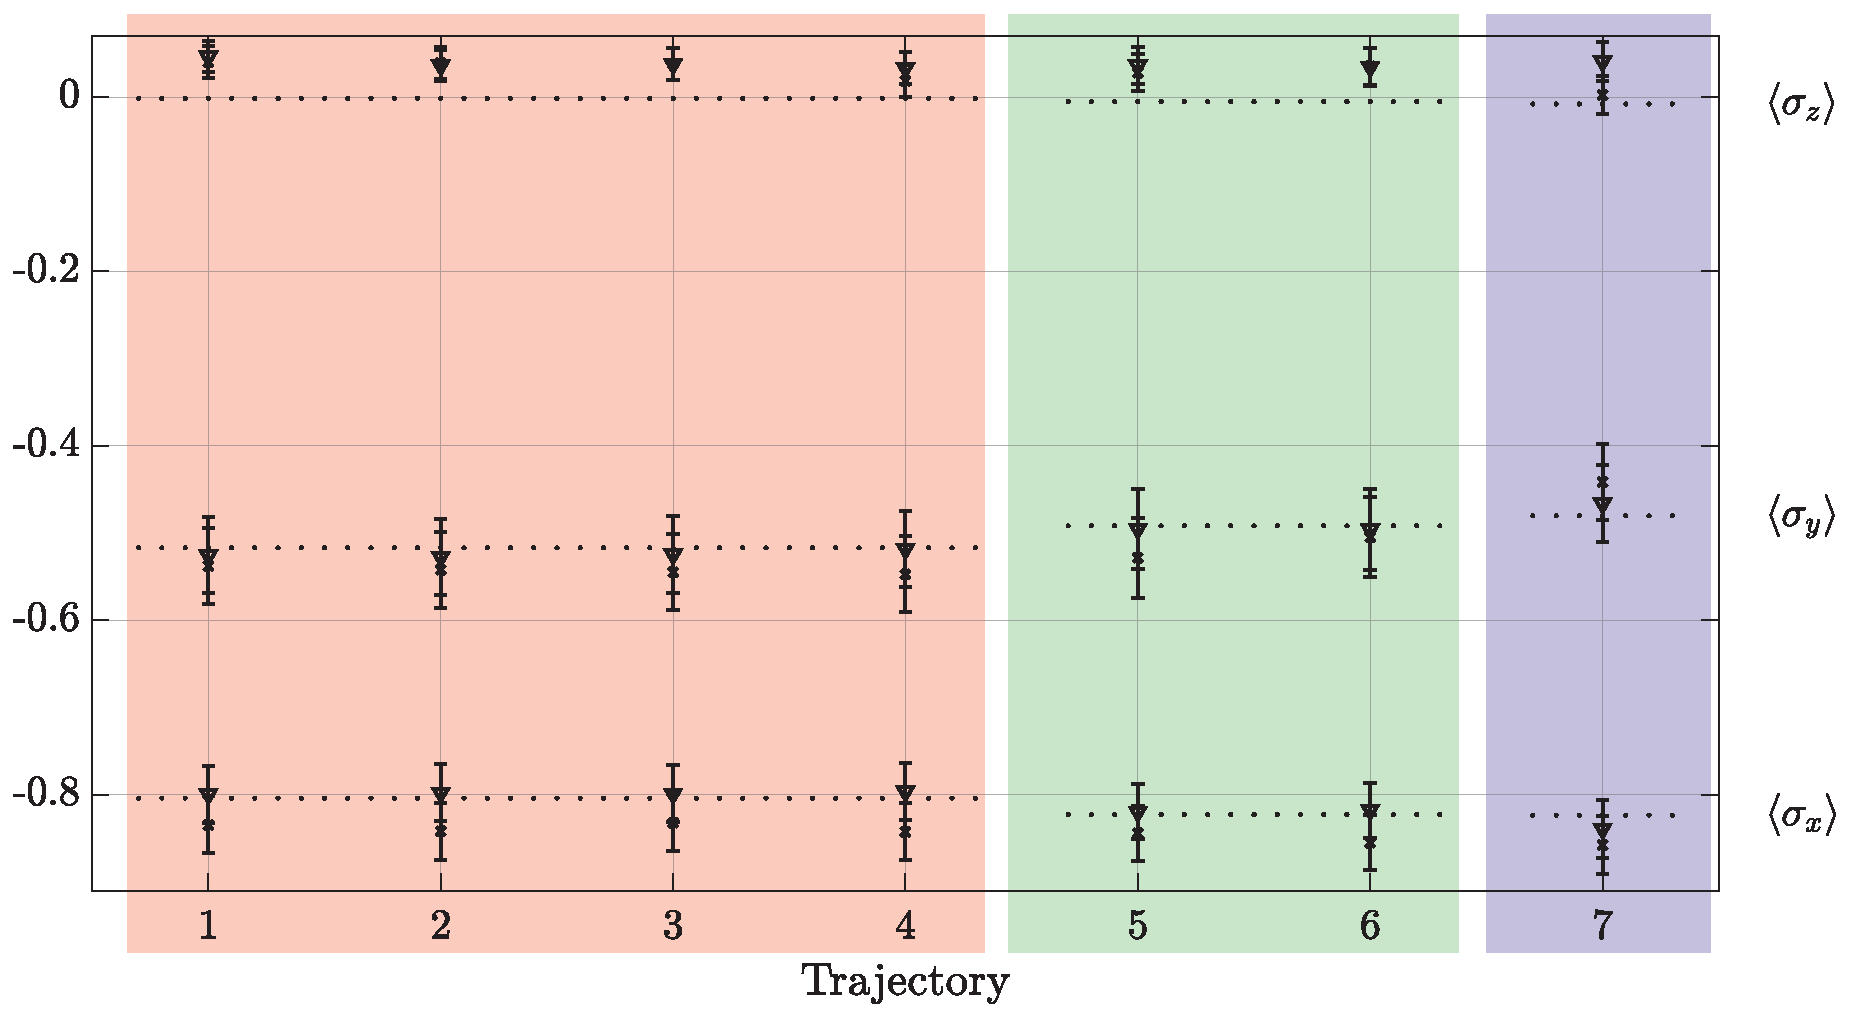
\includegraphics[width=0.85\textwidth]{salida4.pdf}
\caption{Valores medios de los observables de  polarización %Mean values of the polarization observables 
$\langle\sigma_{\mu}
\rangle$ para diferentes evoluciones del estado inicial $|S_0\rangle$. Se comparan los resultados teóricos  ($\circ$) con los valores experimentales obtenidos promediando sobre todas las regiones  ($\times$), y por medio de una \'unica medida ($\blacktriangledown$).}
\begin{tabular}{ccccccccccccccc}
    \hline
{\rm Trayectoria} && 1 && 2 && 3 && 4 && 5 && 6 && 7  \\
    \hline
 {\rm Nº de Estados de tiempo} ($N$) && 2 && 4 && 4 && 8 && 4 && 4 && 8  \\
    \hline
    \end{tabular}
\label{fig:stokes}
\end{figure}

 En la Fig. (\ref{fig:stokes}) se muestran resultados para los valores medios de los observables de polarización obtenidos en distintas trayectorias y por los dos métodos descriptos por la Ec. (\ref{prom}):  promediando los valores medios de medidas secuenciales y por medio de una única medida del estado historia en el plano de Fourier, observándose un buen acuerdo entre ambos métodos. Las distintas trayectorias constan de $2$, $4$ u $8$ estados de tiempo (rendijas), para niveles de gris entre 0 y 40, y los estados de polarización $|S_t\rangle$ de estos estados historia  están expresados en términos de los valores medios de los operadores de Pauli
 $\langle\sigma_\mu\rangle$ (ver \ref{sec:Evolution operators}), los cuales son directamente los parámetros de Stokes medidos que se muestran en la Fig. (\ref{fig:stokes2}).
 
%  \begin{table*}[h!]
%   \centering
% %  \begin{adjustbox}{sc0.8\textwidth}
% \resizebox{\columnwidth}{!}{    \begin{tabular}{|ccccccccccccccccccc|}%ccccccccc|}
% \label{table:8steps}
%     \hline
%   && && && && {\rm Tiempo}&& && && && &&\\
%     \hline
%   && {\rm Trayectoria} &&
% $t_1$ && $t_2$ && $t_3$ && $t_4$ &&$t_5$ && $t_6$ && $t_7$ && $t_8$\\
%     \hline
% %\begin{sideways}Trajectory\end{sideways}
%  {$\langle\sigma_{x}
% \rangle$} &&  &&-0.7110&& -0.3183 && -0.6849 && -0.2957&&-0.3496&&-0.7315&&-0.3432&&-0.7112  \\
%  $\langle\sigma_{y}
% \rangle$ && $\ 1$ &&-0.6614 &&-0.9382  && -0.7017 && -0.9303 &&-0.9180&&-0.6473&&-0.9263&&-0.6475    \\
%  $\langle\sigma_{z}\rangle$ && &&0.0382 && 0.0288 && 0.0433 && 0.0183 && 0.0337 && 0.0376 && 0.0322 && 0.0334  \\
%     \hline
% {$\langle\sigma_{x}
% \rangle$} && &&-0.5458 && -0.3308 && -0.5848 && -0.0965 &&-0.7538&&-0.4772&&-0.2489&&-0.6908   \\
%  $\langle\sigma_{y}
% \rangle$ && $\ 2$ &&-0.8194 &&-0.9408  && -0.8004 && -0.9867 &&-0.6383&&-0.8705&&-0.9656&&-0.6910    \\
%  $\langle\sigma_{z}\rangle$ && && 0.0495 && 0.0387 && 0.0548 && 0.0009 &&0.0595&&0.0447&&0.0315&&0.0473  \\
%  \hline
%  \end{tabular}}
% % \end{adjustbox}
% \end{table*}

\begin{figure}[h!]
\centering
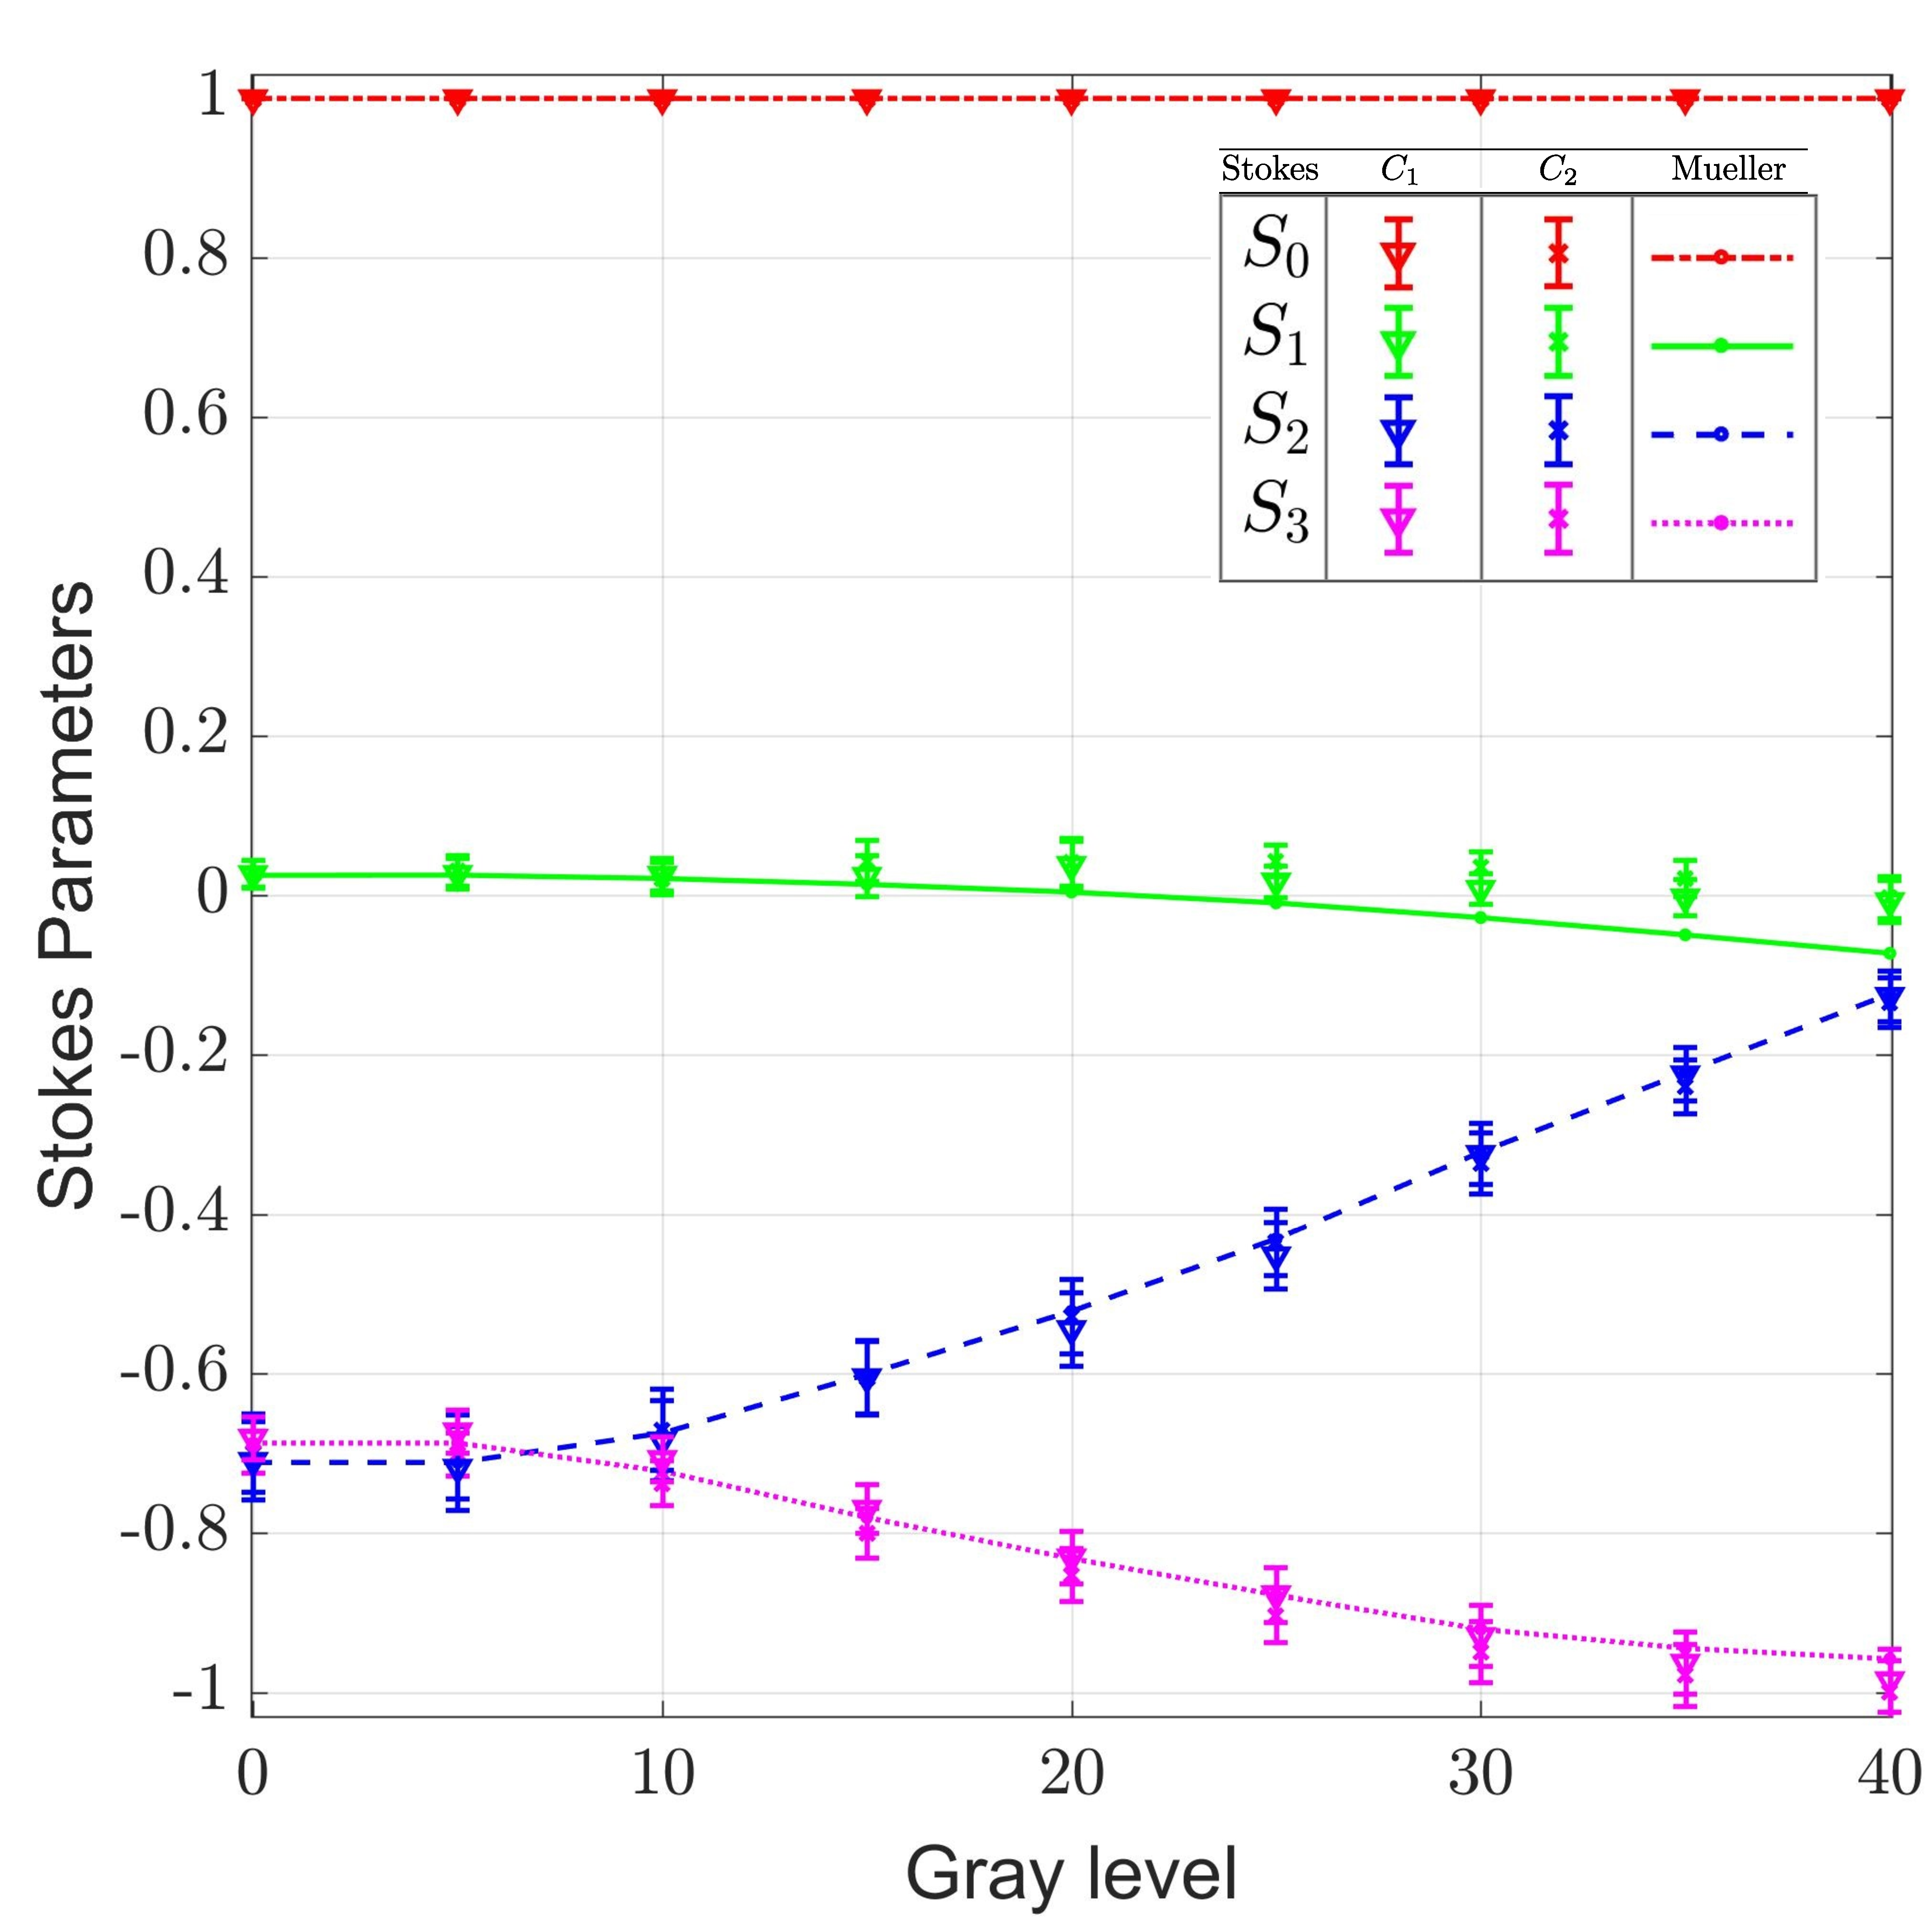
\includegraphics[width=0.85\textwidth]{stokes.pdf}
\caption{Parámetros de Stokes en función del nivel de gris, registrados a través de una cámara {\it CCD} ($C_1$) y una cámara de tecnología {\it CMOS} de alta sensibilidad ($C_2$).A su vez se muestran los resultados obtenidos para las matrices de Mueller para dichos niveles de gris.}
\label{fig:stokes2}
\end{figure}

%%%%%%%%Estado de entrada%%%%%%%%

% \begin{table}[htp]
%   \caption{Estado inicial del sistema
%   %Initial system state $|S_0\rangle$ {\color{red} (ver si esto se expresa segun los parametros de stokes u otro)}
%   }
%   \begin{center}
%     \begin{tabular}{ccccccccccc}
%     \hline
% {$S_0$} && $S_1$ && $S_2$ && $S_3$ && DOP  \\
%     \hline
%  1 && 0.040 && 0.95 && -0.026 && 0.95 \\
%     \hline
%     \end{tabular}
%   \end{center}
% \label{table:mean_val}
% \end{table}

%%%%%%%%%%%%%%%%%%%%%%%%%%% Figure - MEAN VALUES %%%%%%%%%%%%%%%%%%%%%%%%%%%%%%%%


% \begin{table}[htp]
%   \caption{Pureza/ Grado de Polarización ({\it DOP})}

%   \begin{center}
%     \begin{tabular}{ccccccccccccccc}
%     \hline
% {\rm Trajectoria} && 1 && 2 && 3 && 4 && 5 && 6 && 7  \\
%     \hline
%  {\rm Nº de estados de tiempo} ($N$) && 2 && 4 && 4 && 8 && 4 && 4 && 8  \\
% {\rm Pureza} &&  &&  &&  &&  &&   \\
%  $xxx$ &&  &&  &&  &&  &&    \\
%     \hline
%     \end{tabular}
%   \end{center}
% \label{table:mean_val}
% \end{table}

%{\color{red} (.......)}
\bigskip

% En el experimento, como demostracióm de principio, 
%In addition, and as a proof-of-principle demonstration, we 
Con el fin de atenuar el poder del haz láser a nivel de régimen de un fotón, de forma que corresponda a la presencia  de un fotón en promedio, a todo tiempo, en el experimento, se  insertaron filtros neutrales
en el esquema experimental, previos a la etapa {\it PSG}. Esta pseudo fuente puede ser utilizada para simular el  estado de un fotón individual, y es usual en implementaciones ópticas de simulaciones cuánticas o de estimaciones de estados cuánticos \cite{Malik2014,QPS17}.

 En este caso permite  comprobar  la factibilidad del método propuesto para simular las características principales de una evolución cuántica paralela en el tiempo. 
Además, en lugar de una cámara {\it CCD}, se utilizó una cámara de tecnología {\it CMOS} de alta sensibilidad ({\it Andor Zyla 4.2 sCMOS}) para realizar las medidas de intensidad en este régimen. 







%have inserted neutral-density filters, previous to the PSG stage, to highly attenuate the power of the laser beam at the single-photon regime, in such a way, that it corresponds to the presence of less than one photon, on average, at any time, in the experiment.
%This pseudo single-photon source can be used to
%mimic a single-photon state, and 
%as is usual in optical implementations of quantum %simulations or quantum-states estimation 


%to carry out the intensity measurements in this regime.
%it is enough to test the feasibility of the proposed method for simulating the main features of a parallel-in-time quantum evolution. Besides, instead a CCD camera, we used a high sensitive camera based on CMOS
%technology (Andor Zyla 4.2 sCMOS) to carry out the intensity measurements in this regime.

%We show
%that the performance of the method in the present realization is limited by polarization dephasing effects [12], and other
%sources of noise like fluctuations in the phase modulation and
%photon number statistics.

%%%%%%%%%%%%%%%%%%%%%%%%%%% TABLE - Polarization degree %%%%%%%%%%%%%%%%%%%%%%%%%%%%%%%%

%%%%%%%%%%%%%%%%%%%%%%%%%%%%%%%%%%%%%%%%%%%%%%%%%%%%%%%%%%%%%%%%%%%%%%%%%%%%%%

%to reduce the effects of the phase fluctuations
%present in modern liquid crystal on silicon (LCoS)
%displays~\cite{lizana2008}.



%Efectivamente, en un fase dimerizada.



\subsection{\label{sec:Evolution operators} Operadores Evolución y Poder Entrelazante}

Anteriormente en la sección \ref{sec:state_generation}, se indicó que la modulación introducida por el {\it SLM} puede describirse por una transformación unitaria en el espacio de polarización. Experimentalmente, la modulación asociada a un dado nivel de gris en la pantalla se describe por una matriz de Mueller $M$ de $4\times 4$ \cite{marquez2008}. La matriz de Mueller actúa como una transformación lineal en el estado de polarización, el cual se representa por el vector de Stokes $\bm s$, definido como
\begin{equation}
\bm s=\begin{pmatrix}s_0\\  s_1\\ s_2\\ s_3\end{pmatrix}=\begin{pmatrix}P_{00}+P_{\frac{\pi}{2}0}\\  P_{00}-P_{\frac{\pi}{2}0}\\ P_{\frac{\pi}{4}0}+P_{-\frac{\pi}{4}0}\\ P_{\frac{\pi}{4}\frac{\pi}{2}}+P_{-\frac{\pi}{4}\frac{\pi}{2}}\end{pmatrix},
\end{equation}
donde los coeficientes $P_{\theta\phi}$ en el último vector son el resultado de 
seis medidas de polarización: polarización lineal horizontal y vertical $(P_{00},P_{\frac{\pi}{2}0})$, polarización lineal  $45^{\rm o}$ y $135^{\rm o}$ ($P_{\frac{\pi}{4}0}, P_{-\frac{\pi}{4}0}$), y
polarización circular derecha e izquierda
$(P_{\frac{\pi}{4}\frac{\pi}{2}}, P_{-\frac{\pi}{4}\frac{\pi}{2}})$. 
Estas medidas corresponden en el formalismo cuántico a proyecciones sobre estados de polarización  $|P_{\theta\phi}\rangle=\cos(\theta)|H\rangle+e^{i\phi}\sin(\theta)|V\rangle$, por lo que tenemos (dado que  $P_{00}+P_{\frac{\pi}{2}0}=1$),  $s_{1}=\langle\hat{\sigma}_{z}\rangle,\,s_{2}=\langle\hat{\sigma}_{x}\rangle,\,s_{3}=\langle\hat{\sigma}_{y}\rangle$, 
donde $\langle\hat{\sigma}_{\mu}\rangle$ denota el valor medio del 
i-ésimo operador de Pauli definido respecto de la base $\{|H\rangle, |V\rangle\}$. Luego, el estado de polarización del fotón individual está dado por
\begin{equation}
    \rho=\frac{1}{2}\left(\mathbbm{1}+\bm r\cdot\hat{\bm\sigma}\right) 
\end{equation}
con $\bm r=\frac{1}{s_0}(s_1,s_2,s_3)$. Una transformación unitaria en el espacio de polarización corresponde entonces a una rotación del vector de Bloch $\bm r$, 
la cual está asociada a una matriz de Mueller de la forma
\begin{equation}
M_R=\begin{pmatrix}
    1&&\bm 0\\
    \bm 0&& m_R 
    \end{pmatrix} \label{ret}
\end{equation}
donde $m_R$ denota una matriz de rotación arbitraria de $3\times 3$.
Una matriz de Mueller como (\ref{ret}) describe
el efecto de un retardador ideal. Sin embargo, el {\it  SLM}
utilizado en la implementación, modula simultáneamente fase y amplitud, es decir,  
no solo introduce un retraso sino también cierta  atenuación. Por lo tanto, la matriz de Mueller asociada a un dado nivel de gris no tendrá exactamente la forma (\ref{ret}), 
que mapea a una transformación unitaria en el espacio de polarización. No obstante, es posible a partir de la descomposición de Lu-Chipman \cite{Lu.96} extraer una matriz de retardo que tiene en cuenta la transformación de fase introducida por el {\it SLM}.
De esta forma, se obtuvo un conjunto de matrices unitarias efectivas que describen las transformaciones realizadas sobre la polarización del fotón para 54 niveles de gris entre 0 y 255. 
%Este conjunto de unitarias nos permite simular estados historia que no pueden implementarse en presente esquema debido a limitaciones experimentales (se observa una disminución en la pureza del estado para niveles de gris por encima de 40).
En la Fig. \ref{fig:sphere2} se muestran ejemplos de estas evoluciones simuladas para la polarización del fotón como trayectorias en la esfera de Bloch.

\begin{figure}[htp]
\centering
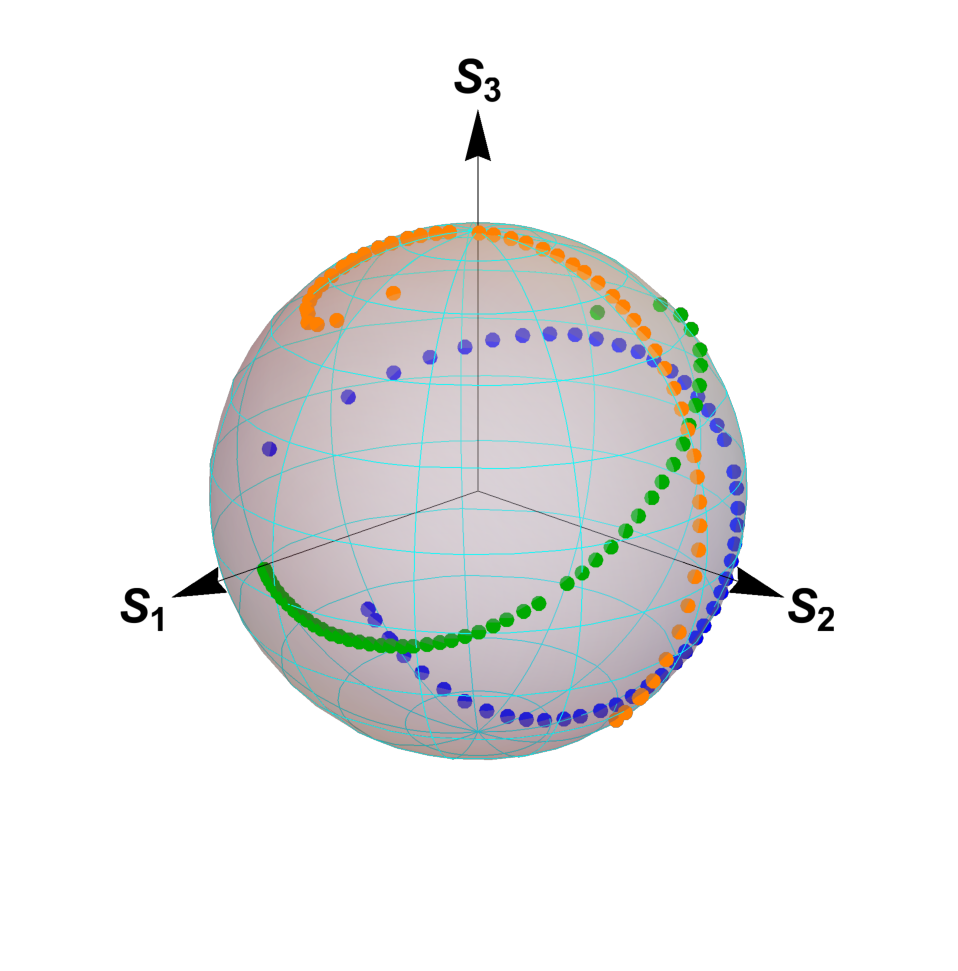
\includegraphics[width=0.6\textwidth]{Figures/SphereF.pdf}
\caption{Simulación de evoluciones para la polarización del fotón como trayectorias en la esfera de Bloch, para tres estados ``semilla'' $|S_0\rangle$ distintos.}
\label{fig:sphere2}
\end{figure}


% Mueller, Descomposición Polar, como se derivan las unitarias

Para cualquiera de estos estados historia simulados podemos reconsiderar al 
operador generador ${\cal W}=\sum_t U_t\otimes |t\rangle\langle t|$, el cual se puede expresar, utilizando su descomposición de Schmidt (ver \ref{Sf})  como 
\begin{equation}
{\cal W}=\sum_t (\frac{1}{2} \sum_{\mu=0}^{3} r_{\mu}(t) \sigma_{\mu}) \otimes |t\rangle\langle t|=\sum_{\mu=0}^{3} \lambda_{\mu}\tilde{\sigma}_{\mu}\otimes O_{\mu}\,.
\end{equation}

En primer lugar se expandieron los operadores unitarios en el espacio de polarización en operadores de Pauli y luego se escribió su correspondiente descomposición de  Schmidt, de acuerdo al formalismo general del capítulo previo,  %descomposición %\cite{BR.18}
 donde
$\tilde{\sigma}_{\mu}$ y $O_{\mu}$ son operadores ortogonales de polarización y espaciales 
(${\rm Tr} (\tilde{\sigma}_{\mu}^{\dagger}\tilde{\sigma}_{\nu})=2\delta_{\mu,\nu}$, ${\rm  Tr}(O_{\mu}^{\dagger}O_{\nu})= N\delta_{\mu,\nu}$). Los números reales $\lambda_{\mu}$ son los coeficientes de Schmidt,
los cuales satisfacen $\sum_{\mu}\lambda_{\mu}^2=1$. Son los valores singulares de la matriz de  $4\times N$, $r_{\mu}(t)/\sqrt{N}$. 

Su entrelazamiento cuadrático, $E_2({\cal W}) = 2(1-\sum_{\mu}\lambda_{\mu}^4)$ es
% We have seen that there is a relation between the entanglement  of the operator ${\cal W}$ and that of the history states it generates, 
%   $|\Psi\rangle=\frac{1}{\sqrt{N}}\sum_{t}U_t|S_0\rangle |t\rangle$.
%  We will here  prove that the quadratic operator entanglement entropy $E_2(U,T)\equiv E_2({\cal W})$, Eq.\ (\ref{E2W}), is 
   proporcional al {\it entangling power} de ${\cal W}$, discutido en el capítulo precedente  (ver \ref{IIIc}) 
%   el cual es e
%   which is the average quadratic entanglement it generates when applied to 
%   initial product states $|S_0\rangle H^{\otimes n}|0\rangle$ ($N=2^n$):  
\begin{equation}
 \langle E_2 (S,T)\rangle=\frac{d_S}{d_S+1}E_2({\cal W})\,, \label{rel}
\end{equation}
donde 
 \begin{equation}
 \langle E_2 (S,T)\rangle=
 \int_{\cal H} 2(1- {\rm Tr}\,\rho_S^2) d S_0\, \label{ME2}
\end{equation}
es el promedio del entrelazamiento cuadrático $E_2(S,T)$
del estado historia sobre todos los estados iniciales $|S_0\rangle$ con medida de Haar $dS_0$. 

Se verificó esta relación considerando el conjunto completo de unitarias de polarización disponibles, las cuales proporcionaron una entropía $ E_2({\cal W})=0.712$. A través de una simulación sobre 1000 estados iniciales, se corroboró la  relación previa con un error menor a 0.01. 



